\documentclass[12pt]{article}
\usepackage{hyperref}
\usepackage[margin=1in]{geometry}
\usepackage{graphicx}
\usepackage{color}
\usepackage[T1]{fontenc}
\usepackage[utf8]{inputenc}
\definecolor{pblue}{rgb}{0.13,0.13,1}
\definecolor{pgreen}{rgb}{0,0.5,0}
\definecolor{pred}{rgb}{0.9,0,0}
\definecolor{pgrey}{rgb}{0.46,0.45,0.48}

\usepackage{listings}
\lstset{language=Java,
  showspaces=false,
  showtabs=false,
  breaklines=true,
  showstringspaces=false,
  breakatwhitespace=true,
  commentstyle=\color{pgreen},
  keywordstyle=\color{pblue},
  stringstyle=\color{pred},
  basicstyle=\ttfamily,
  moredelim=[il][\textcolor{pgrey}]{$$},
  moredelim=[is][\textcolor{pgrey}]{\%\%}{\%\%}
}

\title{\Large Text Encodings, FileIO, and Exceptions }
\author{
	Melvyn Ian Drag
}
\date{\today}


\begin{document}
\maketitle

\begin{abstract}
Tonight we will learn how the ASCII, UTF-8 and UTF-16 text encodings work. Then we will see how they apply to Java File I/O Operations. Finally we will take a quick look at Exceptions in Java, as basic knowledge is required to work with File IO classes.
\end{abstract}

\section{Preliminary Remarks}
Last week we talked about the binary representation of whole numbers in Java
programs. We know that Java uses the two's complement system. Today we talk
about:
\begin{itemize}
\item How your computer stores text data
\item How Java reads text data from your computer
\item How text data is represented internally in java
\item How Java writes text data to your computer
\item Some things that can go wrong when handling text data
\end{itemize}

At the end of the lecture, I hope you will be able to talk somewhat
intelligently about the above topics.

To begin you should know that there are many different binary encodings for text
data on computers. Today we will focus on 3 of the more common ones, but you
must be aware that there are others.

We are going to talk about ASCII, UTF8, and UTF16.

Please before we get started, take a moment to go to
\url{github.com/melvyniandrag} and note the
\textit{TextFilesInDifferentEncodings} repository there. Click the repo. Then
note there is a green button that says "Code". Click that button, then go to
"download zip" and download it. Then unzip it. Start a new Java project in
Eclipse and add the files from the repository to your new project src folder.


\section{Lets Play Around Before We Look At Theory}

I will write the code on the board and ask everyone to create the same class
inside a package called textencodings in the project they just created.
See Figure \ref{fig:environment} to see what your computer should look like.

\lstinputlisting[caption=Read a UTF8 Encoded File]{ScannerExample.java}

\begin{figure}[h]
\centering
	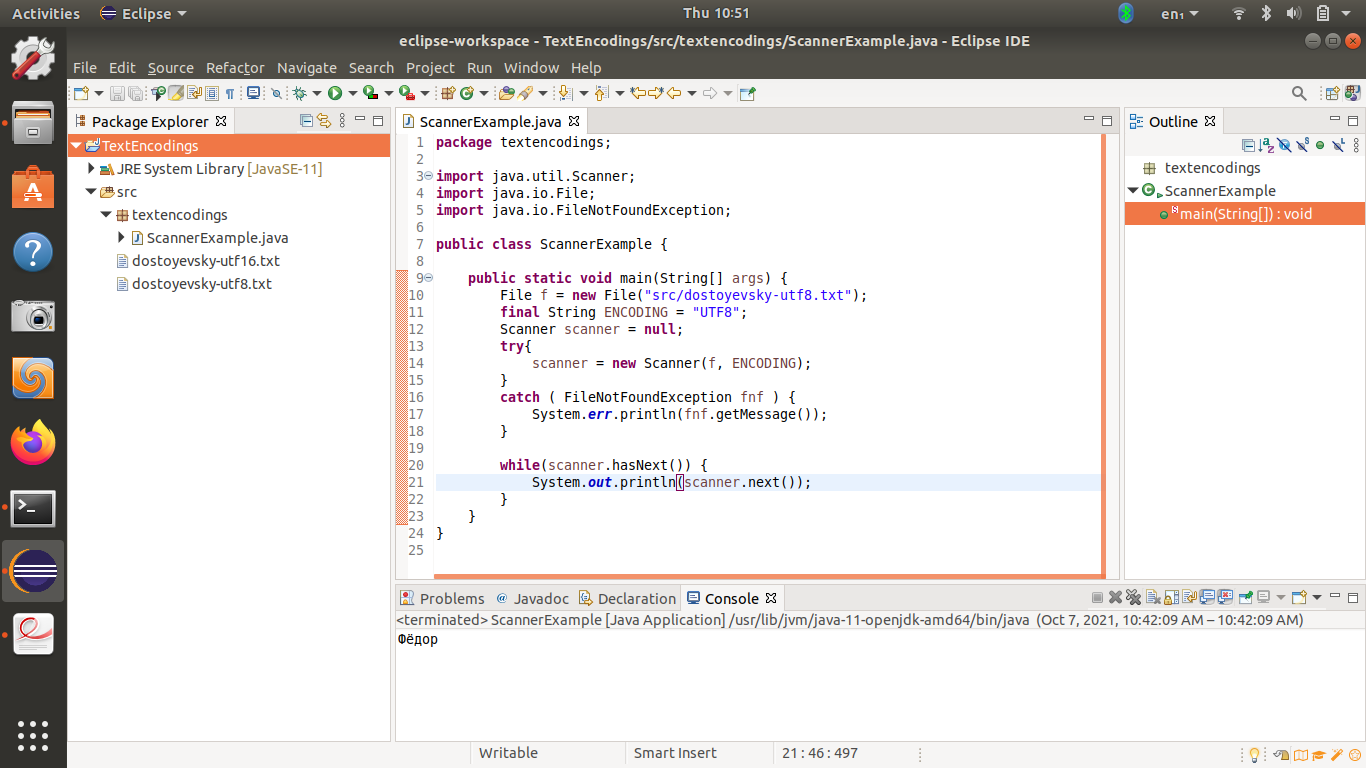
\includegraphics[width=0.8\textwidth]{environment.png}
	\caption{{\small \texttt{What your setup should look like now.}}}
	\label{fig:environment}
\end{figure}


\subsection{Now Do This}
\begin{itemize}
\item change the ENCODING to UTF16 and rerun. The computer prints out junk.
\item Then change the ENCODING to UTF16 and also change the input file to the
one with utf-16 instead of utf-8. Rerun. Now the computer prints out the correc
t thing.
\end{itemize}

\subsection{What Happened?}
There are many different schemes / techniques / styles of storing text data on
computers. I mean to say that the ones and zeros can be rearranged. The format
of the ones and zeros is known as a text encoding. The three we are talking
about are: (audience participation)

\subsection{I'd like to show you one more thing before we talk theory}
Run the dostoyevsky files through xxd on laptop or on lectern pc. xxd is a
command line tool that dumps out file contents in hex.Show that the hex is
different for the dostoyevsky files. Show that the hex is different for the
hello files.


\section{How about one more example?}
Buffered readers can be more efficient than other types of readers when reading
Java programs. File IO is very time consuming - it is the most time consuming
thing for computers. 


Checkout this example that reads a file using a Buffered Reader.
\lstinputlisting[caption=Read a file using a
BufferedReader]{InputStreamExample.java}
 
\section{ASCII}
Many years ago, a short while after the beginning, there was an encoding called "ASCII". You see, the computers and the programmning languages in the beginning were designed in the USA and the UK mainly, and so all of the technology was dealt with in English. This is why the programming languages say ``character'' and ``integer'' and not whatever their equivalents are in other languages. At the same time, math and science publications were moving away from German, French and Russian and everything was being written in English, for ease of international exchange of ideas. 

And so, as this was happening, it is not surprising that computers were designed to represent English language characters, punctuation, numbers, and a few other things needed by a computer. 

\begin{center}
\textbf{hand out ASCII table}
\end{center}

What I am handing to you is a table showing the binary encoding for text in the ASCII system. If your programming language supported ASCII, you would therefore write the character '0' as 0x30. You would represent 'a' as 0x97. The ASCII encoding could do other things too - if you wanted a blank line you could write '\textbackslash n', stored in memory as 0x0A. If you wanted a tab you could write '\textbackslash t', which was stored in memory as a 0x09.

The encoding even featured a way to make your computer make a beeping sound! You can try to print an '\textbackslash a' on your computer ( '\textbackslash a' is stored in memory as 0x07 ) and depending on how your laptop/pc is configured it might still beep. If there is time after class we can try together.

\subsection{ASCII Art}
If you have heard the term ASCII before, there is a good chance that you have heard about it in the context of 'ASCII-art'. Pictures like this are still somewhat popular in certain text circles:

\textbf{Note: In class just go to the url to show the class}

\begin{lstlisting}

      (\-"""-/)
       |     |
       \ ^ ^ /  .-.
        \_o_/  / /
       /`   `\/  |
      /       \  |
      \ (   ) /  |
     / \_) (_/ \ /
    |   (\-/)   |
    \  --^o^--  /
     \ '.___.' /
jgs .'  \-=-/  '.
   /   /`   `\   \
  (//./       \.\\)
   `"`         `"`

\end{lstlisting}

\url{https://www.asciiart.eu/animals/marsupials}

\subsection{ASCII is a Seven Bit Encoding}
Show that the table goes up to 127. On the board, multiply 2x2x2x2x2x2x2 = 128 = 2\^7, with seven bits we get numbers 0-127.

Indeed, ASCII characters are seven bits and so they fit in a single byte. This
is why in certain older programming languages out there the "char" datatype is
one byte - because a character takes up only one byte.

\subsection{Please review the ascii table}
This shows the binary representation of all valid characters from years ago.
ASCII is still popular btw, but that is only because the ancient ASCII encoding
is compatible with a new encoding. The computer scientists who designed this
stuff were very clever.


\subsection{TODO}
What is the ASCII representation of hello?
Note: there is not ASCII representation for fyodor in cyrrillic,because ASCII is
for english letters only.
Leave the ascii neatly on the side of the board.

\section{UTF16}
When ASCII came out, this was many years ago as I told you. In the early 1990s \textit{(Check me out on this, I might be off bya couple of years)}, and at this time personal computers were starting to spread around the world. The computers back then were primitive compared to what we have now \textbf{Show class a picture of the Commodore 64}, but the computers were being used by speakers of many languages. At this time it was becoming very important for people to write in their own native languages. Some people used Cyrillic letters, others used Sanskrit letters, Japanese and Chinese had many many characters, and so on. The ASCII encoding had one bit left over, so by turning on the remaining bit in the encoding there were now 128 new characters that could be represented by ASCII.

\begin{center}
\textbf{Write on board 8 bits, show how putting a 1 in the leading position allowed for 128 new values. For all the old 128 values, there was a new value corresponding to it if you turned the first bit on.}
\end{center}

Do you think that all the alphabets in the world fit in the allocated 128 extra characters? \textit{Wait for a resounding no}.

Different vendors tried different things. You could install different character sets on your computer, each characterset representing different letters, but this was cumbersome. Many different internationalization schemes appeared in the technological world. It's very interesting stuff and if you want to know more you can poke around the internet.

In the early 1990s, and it was about this time that people were clamoring for a standard internationalization scheme so the mess of competing character sets didn't continue to spiral out of control. What was decided was that all characters could be represented - instead of in 8 bits - in 16 bits! The new standard was dubbed unicode, and this implementation was called UTF-16. 

Ive given you two utf16 files right? The ones and zeros in those files follow
the pattern specified in the utf16 specification. I don't know all the rules of
UTF16 off the top of my head. Anyway, there are rules. In ascii an a is 0xXY,
well in utf16 it is 0x00 0xXY - 16 bits instead of 8.

Heres an interesting thing: Java came out in the early 90s. What text encoding
scheme do you think the Java people chose to use for the  Java String and
Character types?

Shortly after the release of Java, after the language designers adopted this 16 bit character for their new, modern language, the standards committee changed it's mind. The Unicode consortium continued on with UTF-16, but they realized that all the characters in the world could not be represented in 16 bits. So the amended the UTF-16 standard such that it would \textit{usually} use 16 bits for characters, but othertimes it would use 32 bits as was necessary.

As such, UTF-16 is known as a variable-width encoding, whereas ASCII was a fixed, 7 bit wide encoding. Do not forget! UTF-16 can hold 2 byte characters, or 4 byte characters.

And so Java, already designed and released to the world, had a 16 bit character type, that was \textit{usually} good enough for text, but sometimes things went haywire.

\section{Exercises}
\subsection{Exercise 1}
How many bytes are in a Character in Java? Instruct the class to write a code to get the number of bytes in a character. Use the \textit{Character.SIZE} member to find out.

Answer: 2 bytes / 16 bits.

\subsection{Exercise 2}
Write and run this code:
\lstinputlisting[caption=string vs byte arraylength]{UTF16Lengths.java}

\section{UTF-16 and Java}
Do not forget! All characters in Java are 16 bits wide. Other programming languages will behave differently - forget everything you know! Java characters are 16 bits wide.

Now we will dip our toes into the mysterious waters of Text Encodings and Java. Run the `StringLength.java' code, found in the class repository.

Have a look at the output. Note that there are two strings, each of length 5. One is written in Russian, the other in English. Nevertheless, Java says the length of each is 5. 

Both strings have a strange "FE FF" in the beginning - ignore that for now. Java reports 12 bytes each, but it's actually 10 bytes plus these extra two weird bytes - we'll just ignore them for a minute.

\begin{center}
\textbf{As a class verify that the utf-16 bytes are correct for both Fyodor and hello.}
Verify the Fyodor bytes using this table:
\url{https://en.wikipedia.org/wiki/Cyrillic_script_in_Unicode#Basic_Cyrillic_alphabet}
\end{center}

\subsection{UTF-16 is the bomb. But the BOM is not.}
The BOM is the "FE FF" we see at the beginning of the byte arrays gotten from the strings. Luckily, Java characters are stored in Big Endian order. That means, that the first byte goes first, then the second byte. As we discussed last week, that is not universally the case. Some UTF-16 methods will come with a "FE FF" or "FF FE" pair of bytes at the beginning. \textbf{This is the twilight zone!!} Sometimes the Byte order mark / BOM is there, sometimes it is not. Tread carefully when you write code that manipulates utf16 text. Sometimes if you get data from a different source, the internet for example, the data will be in Little Endian order. This text will have the BOM/Byte order mark "0xFF, 0xFE". You may need to check this, depending on your use case. 

\subsection{Look at Unicode points U+XXXX syntax}
Have a look here. \url{https://www.fileformat.info/info/unicode/char/0424/index.htm}
Across the internet there are various places where you can find unicode data.
Note that the cyrrillic f is U+0424.

\section{How to write Unicode characters in Java.}

Your keyboard probably only has English characters on it. So how do you write
unicode strings in Java? Note - if you speak Arabic you will probably have an
international keyboard layout that lets you type arabic characters. But then how
do you type Chinese characters with your Arabic keyboard? 

We can write the code points using a special syntax.This syntax is not for any
particular unicode. Note that today we are learning about two flavors of
unicode: UTF8 and UTF16. These code points that we are going to type now are the
same for both. The binary is different, but this representation is the same.
Just like the letter "a" can be ascii, utf8 or utf16.

Here's how you put foreign characters in your Java programs:


\begin{center}
\textit{recordação} 
\end{center}

Hints for the Portuguese letters:
\begin{enumerate}
\item https://www.fileformat.info/info/unicode/char/00e7/index.htm
\item https://www.compart.com/en/unicode/U+00E3
\end{enumerate}

Look up the characters in that reference.


\lstinputlisting[caption=portuguese]{Portuguese.java}

\subsection{Exercise}
Use this reference: https://www.khngai.com/chinese/charmap/tbluni.php?page=0
and make your Java program print out a 15 different chinese characters.

\subsection{Interesting note about the last thing:}
https://chinese.stackexchange.com/questions/16788/is-there-really-no-unicode-for-%E6%89%8C

Note that there are many weird symbols all over the page. This is because the
browser doesnt support the binary for that particular character. So the browser
is trying to display a series of 1s and 0s, but the font it has doesnt have the
right character to draw on the screen.

Consider - just 30 years ago American computers only supported english - ASCII.
But now we have to support all the languages in the world. That means the fonts
we use - Times New Roman, etc ( what are some more fonts?) need to be updated to
contain ways to draw letters in new languages.


\section{Final Jeopardy \& Break Time}
\begin{itemize}
\item What are all the primitive "whole number types" in Java?
\item Are Java integers signer or unsigned?
\item Are Java "whole number" primitives stored in Big Endian or Little Endian Format?
\item Which bit is always the sign bit in "whole number types" in Java?\item What is the BOM in UTF-16 text?
\item Write "hello" in UTF-16LE, and prepend an appropriate BOM.
\end{itemize}

\subsection{One More Fun Thing}
\lstinputlisting[caption=smile]{PrintEmoji.java}


\section{ Checkpoint }
Remember that Java internally stores text data in chars, Characters and Strings in a UTF-16 encoding. Not ASCII. And not any of the other million encodings that exist. Always UTF-16. And always big-endian.

\section{UTF-8}
\subsection{Preamble}

Go to google.com and right click -> view page source. It says UTF8.

Most people use utf8 on the internet. The eclipse IDE stores all data as UTF8.
The code files you write - those are utf8 files! If you convert them to utf16
and try to compile them, they wont work!

The list goes on. Most people are using utf8 these days.

Unfortunately again for Java ( and for Windows as well ), UTF-16 is not a widely used or loved text encoding. If you write a program that ingests data from the internet or desktop applications, the text is probably encoded in what is called "UTF-8". As I  mentioned before, when Java ( and Windows ) came about in the early 1990s, the Unicode consortium was working dilligently to choose the best encoding for international text. And silly things like emojis, and mathematical symbols, etc..

Shortly after they settled on UTF16 being a 16 bit encoding, they decided it should be variable 16/32. Then they decicded it should actually be 8/16/24/32 bits. This new encoding, that ranged from 1 - 4 bytes, was called "UTF-8". 

Before I tell you how UTF-8 works, I'll just tell  you that my laptop ( and yours probably ) has a UTF-8 encoded terminal. Whatever text you see in my terminal is internally encoded as UTF-8. Just as Java used UTF-16. So, returning to that strange thing I showed you before we wnet on break, where I tried to print 0x0080 to the console, but my terminal said I had printing 0xC280 - Well lets look at the Unicode page:
\url{https://www.fileformat.info/info/unicode/char/0080/index.htm}

you will see that in UTF-16 it is encoded as 0x00 0x80, but in UTF-8 it is encoded as 0xC2 0x80.

\subsection{How UTF-8 works}
What I am going to give you now is a cool exerpt from a little hacker journal that's quite popular. I've given you three articles, one which is relevant to today's lecture, one is relevant to your life, and one is relevant to next week's lecture.

\begin{center}
\textbf{Handout POC || GTFO pamphlet}
\end{center}

Take a minute to skim through this now and see if anything in there makes sense to you ( allow 2 minutes ). Now, soon you'll be able to read article one. Maybe not tonigh, but definitely after doing the homework you'll be able to read article one and make some sense of what they're talking about. Article 2 is a great read for people who like doing crafts and projects. Article 3 is likely to go over your head, but you can skim it to set the stage for next week's lecture.

Anyway let's return to lecture. UTF-8 is one of the coolest encoding schemes in the world. It is a variable width encoding, but it has some nice properties that make it easy to parse as a computer.

UTF-8 is great because it is compatible with ASCII! All one-byte UTF-8 characters are valid ASCII characters. So now you understand about half of how UTF-8 works. If you look on Page XXXX of the pamphlet I just gave you you'll find a table explaining how UTF-8 works. Note that the one byte charactrs are just like ASCII. Remember that ASCII is a seven bit encoding with a zero in the first position. I've given you an ASCII table - if you have time later you can choose a few of those hex values and convert them to binary and you'll see they all start with a leading zero.

\begin{center}
\textbf{write on board the one byte UTF-8 boiler plate}
\textit{Note that we have 7 bits ( the xs ) to represent our code point. Any code point that needs to convey only 7 bits of info will fit there}
\end{center}

Now, how does UTF8 work for larger UTF code points?

Note the positions of the xs, ys and zs in the table I gave you for UTF8, the table in the pamphlet.

UTF-8 is a prefix encoding. 

The rules:
\begin{enumerate}
\item If the code point is one byte long, start the byte with a zero.
\item If the code point is two bytes long, start the first byte with 2 ones, then a zero, the your data. The second byte must start with '10'
\item If the code point is three bytes long, start the first byte wit 3 ones, then a zero, then your data. The second and third bytes start with '10'
\item If the code point is four bytes long, start the first byte with 4 ones, then a zero, then your data. The second, third and fourth bytes start with '10'
\end{enumerate}

The rules ( part 2):
\begin{enumerate}
\item Get the hex value for the Unicode code point you want to encode in UTF-8 ( That's the U+XXXX(y?) value.)
For the treble clef, the code point was \textbf{U+1D11E}. Note we are using the value associated with the big U.
\item Convert the hex after the U+ to binary
\item See how many binary digits it requires
\item See if you will need 1, 2, 3, or 4 UTF-8 code points to accomodate that many digits. 
\item Starting from the left, fill the blank spaces in the UTF-8 boiler plat with the binary digits from the code point you just wrote in binary.
\item If there are any left over places, fill with zeros.
\item Done. Convert to hex if you want.
\end{enumerate}

\begin{lstlisting}
0x1D11E = 0b11101000100011110 (17 bits)
One byte UTF-8 gives 7 free bits for data
Two bytes give 11 free bits
Three bytes give 16 free bits
So we must use 4 bytes, which gives 21 free bits.
Now we just fill in:
1111XXXX 10XXXXXX 10XXXXXX 10XXXXXX
11110000 100XXXXX 10XXXXXX 10XXXXXX // pad with zeros, we only need 17 bits
11110000 10011101 10000100 10011110 // Fill in the 17 bits from the U+1D11E

11110000:10011101:10000100:10011110 // VERIFY AGAINST https://www.fileformat.info/info/unicode/char/1d11e/index.htm
\end{lstlisting}


\subsection{Exercise}
There is a language spoken in Southeast Asia calle \textit{Tamil}.
One of the letters of the alphabet is the one given here: \url{https://www.fileformat.info/info/unicode/char/0b8a/index.htm}

The unicode code point is U+0B8A. Convert this code point to UTF-8 and verify your answer with the answer online.


\section{Writing Files in Java}
I gave you two ways to read files before. And I gave you a bunch of information
about ASCII, UTF8 and UTF16. I need to tell you a few ways to write files out in
different text encodings. You might want to write your file data as utf8, you
might want utf16, you might want something else.

\subsection{Oneway}
\lstinputlisting[caption=With Files.write]{SimpleWriter.java}

\subsection{Another way}
\lstinputlisting[caption=With OutputStreamWriter]{OutputStreamWriterExample.java}


\section{Exceptions}
Java is a language that has exceptions. If something goes wrong, Java can throw
an exception instead of just crashing the program. You can catch the exception
and do something with it. 

For example, in this class we've see :
FileNotFoundException.

If you try to read a file that isn't there - what should happen? One valid thing
to do is just crash the program. But that's kind of bad - you wont know what
went wrong! So Java lets you catch(FileNotFoundException ex) and then read what
went wrong System.err.println(ex.getMessage()). There are more things to know
about exceptions. The throws keyword, try/catch/finally. For now we will just do
Try/Catch and the check out ex.getMEssage. The exception has more information
too like a stacktrace and other things. Feel free to explore the API!


\section{Review}
Revisit the learning objectives from the beginning. Did we learn anything?

\end{document}
